\subsection{Interaction forte}\label{chapter-MS-MSSM-section-formalisme-subsec-QCD}
\subsubsection{La couleur}\label{chapter-MS-MSSM-section-formalisme-subsec-QCD-subsubsec-couleur}
L'interaction forte est la troisième force fondamentale décrite par le modèle standard.
L'analogue de la charge électrique pour l'interaction électromagnétique est, dans le cas de l'interaction forte, la \og couleur \fg,
concept né de l'observation des baryons \Deltabaryonplusplus, \Deltabaryonminus, \Omegabaryonminus.
Dans le modèle des quarks, ces baryons sont composés comme
\begin{equation}
\Deltabaryonplusplus = (\quarku\quarku\quarku)
\msep
\Deltabaryonminus = (\quarkd\quarkd\quarkd)
\msep
\Omegabaryonminus = (\quarks\quarks\quarks)
\mend
\end{equation}
Or, ces baryons sont de spin $\frac{3}{2}$. Les quarks possédant un spin $\frac{1}{2}$, il faudrait alors que pour chacun de ces baryons, les trois quarks les composant aient leurs nombres quantiques égaux, ce qui va à l'encontre du principe de Pauli.
\par Il est possible de décrire ces baryons sans violer le principe d'exclusion de Pauli en introduisant un nouveau nombre quantique, la couleur. Les quarks portent ainsi une charge de couleur, pouvant prendre trois valeurs orthogonales que l'on nomme par convention rouge, vert et bleu. Les antiquarks portent une anticouleur. Il suffit alors que chaque quark porte une couleur différente, \ie
\begin{equation}
\Deltabaryonplusplus = ({\color{red}\quarku}{\color{green}\quarku}{\color{blue}\quarku})
\msep
\Deltabaryonminus = ({\color{red}\quarkd}{\color{green}\quarkd}{\color{blue}\quarkd})
\msep
\Omegabaryonminus = ({\color{red}\quarks}{\color{green}\quarks}{\color{blue}\quarks})
\mend
\end{equation}
\par Les baryons ainsi formés de trois quarks (un rouge, un vert et un bleu) portent une charge de couleur globale nulle, ils sont de couleur \og blanche \fg, comme cela est visible sur la figure~\ref{subfig-colors_for_baryons}. Dans le cas des antibaryons formés de trois antiquarks, sur la figure~\ref{subfig-colors_for_antibaryons}, c'est l'association des trois anticouleurs qui permet d'obtenir un baryon blanc.
Il est également possible de former une particule composite blanche par association d'un quark avec un antiquark portant l'anticouleur correspondante. Les trois combinaisons possibles sont illustrées sur la figure~\ref{subfig-colors_for_mesons}. Il s'agit alors de mésons.
\begin{figure}[h]
\centering
\subcaptionbox{Un baryon est constitué de trois quarks, un de chaque couleur.\label{subfig-colors_for_baryons}}[.3\textwidth]
{\begin{tikzpicture}
\def\rcircle{1.5}
\def\overlappct{.6}

\fill [ltcolorred2] (90:\overlappct*\rcircle) circle (\rcircle);
\fill [ltcolorblue2] (90-120:\overlappct*\rcircle) circle (\rcircle);
\fill [ltcolorgreen2] (90+120:\overlappct*\rcircle) circle (\rcircle);

\begin{scope}
\clip (90:\overlappct*\rcircle) circle (\rcircle);
\clip (90+120:\overlappct*\rcircle) circle (\rcircle);
\fill [ltcoloryellow2] (90:\overlappct*\rcircle) circle (\rcircle);
\end{scope}

\begin{scope}
\clip (90:\overlappct*\rcircle) circle (\rcircle);
\clip (90-120:\overlappct*\rcircle) circle (\rcircle);
\fill [ltcolormagenta2] (90:\overlappct*\rcircle) circle (\rcircle);
\end{scope}

\begin{scope}
\clip (90-120:\overlappct*\rcircle) circle (\rcircle);
\clip (90+120:\overlappct*\rcircle) circle (\rcircle);
\fill [ltcolorcyan2] (90-120:\overlappct*\rcircle) circle (\rcircle);
\end{scope}

\begin{scope}
\clip (90:\overlappct*\rcircle) circle (\rcircle);
\clip (90-120:\overlappct*\rcircle) circle (\rcircle);
\clip (90+120:\overlappct*\rcircle) circle (\rcircle);
\fill [white] (90-120:\overlappct*\rcircle) circle (\rcircle);
\end{scope}

\draw (90:\overlappct*\rcircle+.5*\rcircle) node {rouge} ;
\draw (90-120:\overlappct*\rcircle+.5*\rcircle) node [rotate=60] {bleu} ;
\draw (90+120:\overlappct*\rcircle+.5*\rcircle) node [rotate=-60] {vert} ;

%\draw (-90:\overlappct*\rcircle+0*\rcircle) node {antirouge} ;
%\draw (-90-120:\overlappct*\rcircle+0*\rcircle) node [rotate=60] {antibleu} ;
%\draw (-90+120:\overlappct*\rcircle+0*\rcircle) node [rotate=-60] {antivert} ;

\draw (0,0) node {blanc};

\def\rcircle{1.5}
\def\overlappct{.6}

\draw (30:\overlappct*\rcircle)+(0, \rcircle) coordinate (top);
\draw (-150:\overlappct*\rcircle)+(0, -\rcircle) coordinate (bottom);
\end{tikzpicture}}
\hfill
\subcaptionbox{Un méson est constitué d'un quark et d'un antiquark de l'anticouleur correspondante.\label{subfig-colors_for_mesons}}[.3\textwidth]
{\begin{tikzpicture}
\def\rcircle{.6}
\def\overlappct{.9}
\def\Dypct{2.5}

\draw (90:\Dypct*\rcircle) coordinate (r);
\draw (-150:\Dypct*\rcircle) coordinate (g);
\draw (-30:\Dypct*\rcircle) coordinate (b);

\fill [ltcolorred2] (r)+(-\overlappct*\rcircle/2,0) circle (\rcircle);
\fill [ltcolorgreen2] (g)+(-\overlappct*\rcircle/2,0) circle (\rcircle);
\fill [ltcolorblue2] (b)+(-\overlappct*\rcircle/2,0) circle (\rcircle);

\fill [ltcolorcyan2] (r)+(\overlappct*\rcircle/2,0) circle (\rcircle);
\fill [ltcolormagenta2] (g)+(\overlappct*\rcircle/2,0) circle (\rcircle);
\fill [ltcoloryellow2] (b)+(\overlappct*\rcircle/2,0) circle (\rcircle);

\foreach \pos in {r, g, b}{
\begin{scope}
\clip (\pos)+(-\overlappct*\rcircle/2,0) circle (\rcircle);
\clip (\pos)+(\overlappct*\rcircle/2,0) circle (\rcircle);
\fill [white] (\pos)+(\overlappct*\rcircle/2,0) circle (\rcircle);
\end{scope}
%\draw (\pos) node {blanc} ;
}

%\draw (r)+(-\overlappct*\rcircle/2,0) node {rouge} ;
%\draw (b)+(-\overlappct*\rcircle/2,0) node {bleu} ;
%\draw (g)+(-\overlappct*\rcircle/2,0) node {vert} ;
%
%\draw (r)+(\overlappct*\rcircle/2,0) node {antirouge} ;
%\draw (b)+(\overlappct*\rcircle/2,0) node {antibleu} ;
%\draw (g)+(\overlappct*\rcircle/2,0) node {antivert} ;

\def\rcircle{1.5}
\def\overlappct{.6}

\draw (30:\overlappct*\rcircle)+(0, \rcircle) coordinate (top);
\draw (-150:\overlappct*\rcircle)+(0, -\rcircle) coordinate (bottom);
\end{tikzpicture}}
\hfill
\subcaptionbox{Un antibaryon est constitué de trois antiquarks, un de chaque anticouleur.\label{subfig-colors_for_antibaryons}}[.3\textwidth]
{\begin{tikzpicture}
\def\rcircle{1.5}
\def\overlappct{.6}

\fill [ltcolorcyan2] (-90:\overlappct*\rcircle) circle (\rcircle);
\fill [ltcolormagenta2] (-90+120:\overlappct*\rcircle) circle (\rcircle);
\fill [ltcoloryellow2] (-90-120:\overlappct*\rcircle) circle (\rcircle);

\begin{scope}
\clip (-90:\overlappct*\rcircle) circle (\rcircle);
\clip (-90-120:\overlappct*\rcircle) circle (\rcircle);
\fill [ltcolorgreen2] (-90:\overlappct*\rcircle) circle (\rcircle);
\end{scope}

\begin{scope}
\clip (-90:\overlappct*\rcircle) circle (\rcircle);
\clip (-90+120:\overlappct*\rcircle) circle (\rcircle);
\fill [ltcolorblue2] (-90:\overlappct*\rcircle) circle (\rcircle);
\end{scope}

\begin{scope}
\clip (-90+120:\overlappct*\rcircle) circle (\rcircle);
\clip (-90-120:\overlappct*\rcircle) circle (\rcircle);
\fill [ltcolorred2] (-90+120:\overlappct*\rcircle) circle (\rcircle);
\end{scope}

\begin{scope}
\clip (-90:\overlappct*\rcircle) circle (\rcircle);
\clip (-90+120:\overlappct*\rcircle) circle (\rcircle);
\clip (-90-120:\overlappct*\rcircle) circle (\rcircle);
\fill [white] (-90+120:\overlappct*\rcircle) circle (\rcircle);
\end{scope}

\draw (-90:\overlappct*\rcircle+.5*\rcircle) node {antirouge} ;
\draw (-90+120:\overlappct*\rcircle+.5*\rcircle) node [rotate=-60] {antivert} ;
\draw (-90-120:\overlappct*\rcircle+.5*\rcircle) node [rotate=60] {antibleu} ;

%\draw (90:\overlappct*\rcircle+0*\rcircle) node {rouge} ;
%\draw (90+120:\overlappct*\rcircle+0*\rcircle) node [rotate=-60] {vert} ;
%\draw (90-120:\overlappct*\rcircle+0*\rcircle) node [rotate=60] {bleu} ;

\draw (0,0) node {blanc};
\end{tikzpicture}}
\caption[Combinaisons des couleurs des quarks dans les hadrons.]{Combinaisons des couleurs des quarks dans les hadrons. La couleur globale est toujours blanche, \ie\ que la charge de couleur globale est nulle.}
\label{fig-colors_for_hadrons}
\end{figure}
\par Les quarks et antiquarks se regroupent ainsi en particules composites, les hadrons (baryons et mésons), dont la neutralité de couleur est confirmée expérimentalement. Ce phénomène est connu sous le nom de \og confinement de couleur \fg{} et est abordé dans la section~\ref{chapter-MS-MSSM-section-formalisme-subsec-QCD-subsubsec-confinement}.
\subsubsection{Symétrie $SU(3)_C$}\label{chapter-MS-MSSM-section-formalisme-subsec-QCD-subsubsec-SU3C}
Afin de décrire l'interaction forte dans le même formalisme que les autre interactions fondamentales, il nous faut un groupe de symétrie. Étant donné qu'il existe trois dimensions de couleur (rouge, verte, bleue), la théorie quantique des champs associée à l'interaction forte se base sur le groupe $SU(3)_C$, où $C$ signifie \og couleur \fg.
\par Tout comme $SU(2)$, $SU(3)$ est un groupe non abélien. Il est possible de reprendre exactement les mêmes calculs que ceux de la section~\ref{chapter-MS-MSSM-section-formalisme-subsec-EW-SU2_general}, en procédant aux changements\footnote{La constante de couplage pour l'interaction forte est souvent notée $\alpha_s$. Nous utilisons ici la notation $g_s$ afin d'illustrer le rôle analogue avec celui $g_Y$ et $g_I$.}
\begin{equation}
\bm{\tau} \in \mathcal{M}_2(\mathbb{C})^3 \leftrightarrow \bm{\lambda} \in \mathcal{M}_3(\mathbb{C})^8
\msep
\bm{\alpha}\in\mathbb{R}^3 \leftrightarrow \bm{\theta}\in\mathbb{R}^8
\msep
g_I \leftrightarrow g_s
\msep
\bm{W}_\mu \leftrightarrow \bm{G}_\mu
\msep
\bm{W}_{\mu\nu} \leftrightarrow \bm{G}_{\mu\nu}
\label{eq-hapter-MS-MSSM-section-formalisme-subsec-QCD-subsubsec-SU3C-analogieSU2}
\end{equation}
où $\bm{\lambda}$ est un vecteur à huit composantes, chacune étant une matrice de Gell-Mann, définies dans l'annexe~\ifref{annexe-maths}{\ref{annexe-maths}}{A} et où $\bm{G}_\mu$ décrit donc huit gluons, bosons vecteurs de l'interaction forte.
\par Les gluons portent une couleur et une anticouleur. Lors de chaque interaction, la charge de couleur est conservée, ainsi un quark rouge interagissant avec un gluon bleu-antirouge devient un quark bleu. Le flux de couleur ainsi conservé dans cet exemple est représenté sur la figure~\ref{fig-fgraph-QCD_color_flux}.
\begin{figure}[h]
\centering
\vspace{\baselineskip}
\subcaptionbox{Diagramme de Feynman de l'interaction.\label{subfig-fgraph-qgqg}}[.3\textwidth]
{\begin{fmffile}{qgq}\fmfstraight
\begin{fmfchar*}(20,20)
  \fmfleft{i1,i2}
  \fmfright{o1}
  \fmf{fermion}{i2,v,o1}
  \fmf{gluon}{i1,v}
  \fmflabel{\gluon}{i1}
  \fmflabel{\quark}{i2}
  \fmflabel{\quark}{o1}
  \fmfdot{v}
\end{fmfchar*}
\end{fmffile}\vspace{\baselineskip}}
\hfill
\subcaptionbox{Représentation du flux de couleur conservé.\label{subfig-fgraph-qgq_colors}}[.3\textwidth]
{\begin{fmffile}{qgq_colors}\fmfstraight
\begin{fmfchar*}(20,20)
  \fmfleft{i1,i2}
  \fmfright{o1}
  \fmf{phantom}{i2,v,o1}
  \fmf{phantom}{i1,v}
  \fmflabel{\gluon}{i1}
  \fmflabel{\quark}{i2}
  \fmflabel{\quark}{o1}
  \fmffreeze
  \fmf{fermion, fore=red}{v,i1}
  \fmf{fermion, fore=red}{i2,v}
  \fmf{fermion, fore=blue}{v,o1}
  \fmfi{fermion, fore=blue}{vpath (__i1,__v) shifted (thick*(2,0))}
  \fmfblob{.2w}{v}
\end{fmfchar*}
\end{fmffile}\vspace{\baselineskip}}
\hfill
\subcaptionbox{Interprétation en utilisant les anticouleurs.\label{subfig-fgraph-qgq_colors_and_anticolors}}[.3\textwidth]
{\begin{fmffile}{qgq_colors_and_anticolors}\fmfstraight
\begin{fmfchar*}(20,20)
  \fmfleft{i1,i2}
  \fmfright{o1}
  \fmf{phantom}{i2,v,o1}
  \fmf{phantom}{i1,v}
  \fmflabel{\gluon}{i1}
  \fmflabel{\quark}{i2}
  \fmflabel{\quark}{o1}
  \fmffreeze
  \fmf{fermion, fore=green+blue}{i1,v}
  \fmf{fermion, fore=red}{i2,v}
  \fmf{fermion, fore=blue}{v,o1}
  \fmfi{fermion, fore=blue}{vpath (__i1,__v) shifted (thick*(2,0))}
  \fmfblob{.2w}{v}
\end{fmfchar*}
\end{fmffile}\vspace{\baselineskip}}

\caption[Interaction entre un quark et un gluon.]{Interaction entre un quark rouge et un gluon bleu-antirouge, donnant un quark bleu.}
\label{fig-fgraph-QCD_color_flux}
\end{figure}

\par Le terme non linéaire $\bm{G}_\mu\wedge\bm{G}_\nu$ dans l'expression de $\bm{G}_{\mu\nu}$\footnote{Obtenue à partir de l'analogie~\eqref{eq-hapter-MS-MSSM-section-formalisme-subsec-QCD-subsubsec-SU3C-analogieSU2} appliquée à l'équation~\eqref{eq-chapter-MS-MSSM-section-formalisme-subsec-EW-defWmunu}.} est lourd de conséquences.
Il permet le couplage entre trois et quatre gluons, comme cela est illustré sur la figure~\ref{fig-fgraph-QCD_3_et_4_gluons}, et donne à l'interaction forte toute sa singularité. En effet, ce terme est responsable de l'initiation de la gerbe partonique qui donne naissance aux jets, dont il est question au chapitre~\ifref{chapter-JERC}{\ref{chapter-JERC}}{sur la calibration en énergie des jets}, ainsi que du confinement de couleur.
\begin{figure}[h]
\centering
\vspace{\baselineskip}
\subcaptionbox{\label{subfig-fgraph-ggg}}[.45\textwidth]
{\begin{fmffile}{ggg}\fmfstraight
\begin{fmfchar*}(20,20)
  \fmfleft{i1}
  \fmfright{o1,o2}
  \fmf{gluon}{i1,v}
  \fmf{gluon}{o1,v}
  \fmf{gluon}{o2,v}
  \fmfdot{v}
  \fmflabel{\gluon}{i1}
  \fmflabel{\gluon}{o1}
  \fmflabel{\gluon}{o2}
\end{fmfchar*}
\end{fmffile}\vspace{\baselineskip}}
\hfill
\subcaptionbox{\label{subfig-fgraph-gggg}}[.45\textwidth]
{\begin{fmffile}{gggg}\fmfstraight
\begin{fmfchar*}(20,20)
  \fmfleft{i1,i2}
  \fmfright{o1,o2}
  \fmf{gluon}{i1,v}
  \fmf{gluon}{i2,v}
  \fmf{gluon}{o1,v}
  \fmf{gluon}{o2,v}
  \fmfdot{v}
  \fmflabel{\gluon}{i1}
  \fmflabel{\gluon}{i2}
  \fmflabel{\gluon}{o1}
  \fmflabel{\gluon}{o2}
\end{fmfchar*}
\end{fmffile}\vspace{\baselineskip}}

\caption{Diagrammes de Feynman correspondant à l'interaction entre trois et quatre gluons.}
\label{fig-fgraph-QCD_3_et_4_gluons}
\end{figure}
\subsubsection{Confinement de couleur et liberté asymptotique}\label{chapter-MS-MSSM-section-formalisme-subsec-QCD-subsubsec-confinement}
Le confinement de couleur force les quarks, particules colorées, à s'associer en formant des particules composites, les hadrons, états liés de charge globale de couleur nulle. Ce phénomène empirique peut s'expliquer par la variation, en fonction de l'échelle d'énergie, de la constante de couplage de l'interaction forte $g_s$, représentée sur la figure~\ref{fig-g_s_fct_energy}.
\begin{figure}[h]
\centering
\begin{tikzpicture}
\node[anchor=south west,inner sep=0] at (0,0) {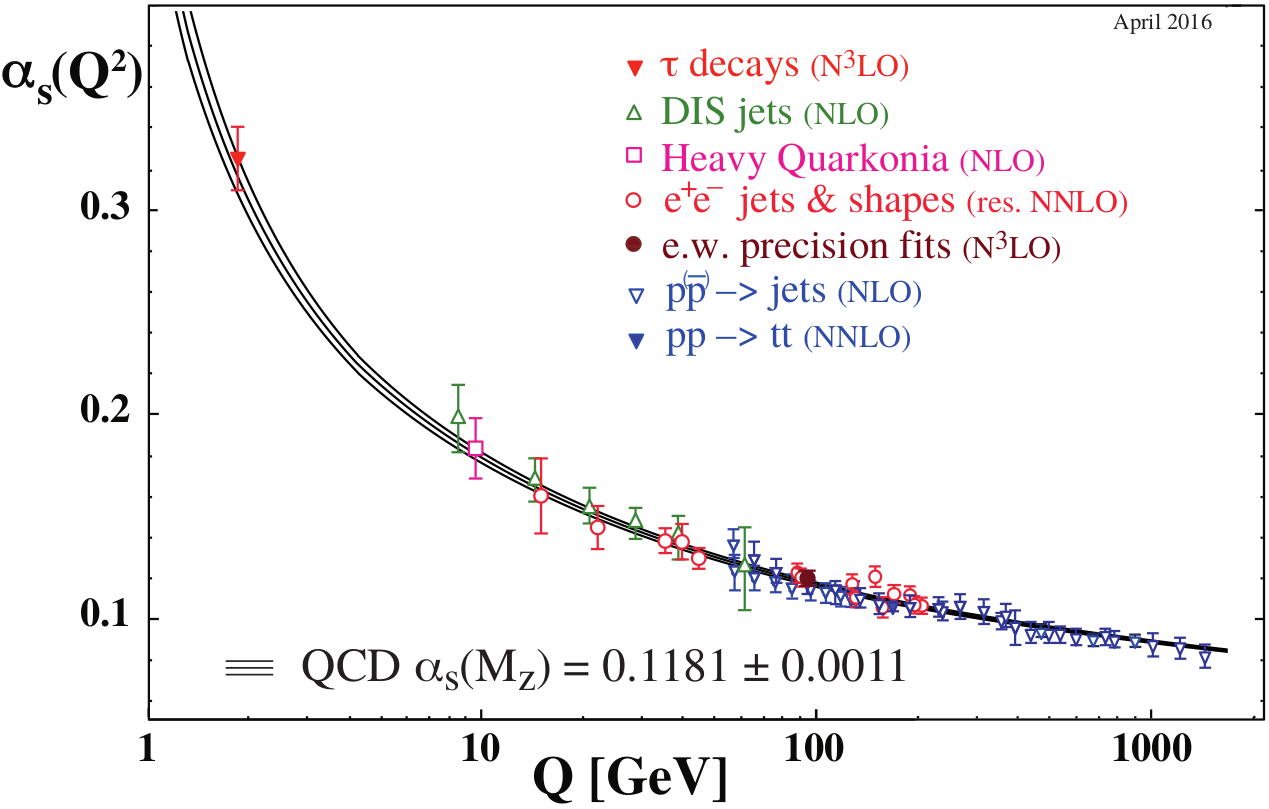
\includegraphics[width=10cm]{\PhDthesisdir/contents/chapter-MS-MSSM/formalisme/QCD_value_fct_Q.png}};
\fill [white] (1,0) rectangle (10, .65);
\fill [white] (1.15,0) rectangle (0,6);
\fill [white] (1.5,.85) rectangle (7.2,1.3);

\draw (1.2,.5) node {\small \num{1}} ;
\draw (3.8,.5) node {\small \num{10}} ;
\draw (6.45,.5) node {\small \num{100}} ;
\draw (9.1,.5) node {\small \num{1000}} ;

\draw (5,.25) node {$k$ (\SI{}{\GeV})} ;

\draw (.8,1.5) node {\small \num{0.1}} ;
\draw (.8,3.15) node {\small \num{0.2}} ;
\draw (.8,4.7) node {\small \num{0.3}} ;

\draw (.5,5.8) node {$g_s(k)$} ;

\draw (1.6, 1.1) node [right] {\small $\equiv$ QCD $g_s(m_{\Zboson}) = \num{0.1181}\pm\num{0.0011}$};
\end{tikzpicture}
\caption[Mesure de $g_s$ en fonction de l'échelle d'énergie.]{Mesures de $g_s$ en fonction de l'échelle d'énergie $k$ (points) et prédiction théorique (courbe)~\cite{PDG_booklet_2018}. Le degré des calculs perturbatifs de QCD utilisés pour extraire $g_s$ est indiqué entre parenthèses (NLO: \emph{next-to-leading order}, \ie\ jusqu'à l'ordre suivant le premier degré non nul; NNLO: un ordre de plus que NLO; etc.).}
\label{fig-g_s_fct_energy}
\end{figure}
\par Aux basses énergie, $g_s$ diverge.
Ainsi, séparer et isoler des particules colorées mène à une énergie potentielle de couleur suffisamment grande pour créer des paires quark-antiquark. Ce processus se poursuit alors jusqu'à ce qu'il ne reste plus que des particules blanches. Lorsqu'un quark est issu d'une collision en physique des particules, ce processus se réalise et s'appelle \emph{hadronisation}. Il s'agit d'une étape de la formation des jets, flux collimé de particules caractéristique de la production de quarks.
\par De plus, à cause de la valeur élevée de $g_s$ aux basses énergies, il n'est pas possible de réaliser des calculs perturbatifs pourtant usuels en théorie quantique des champs.
D'autres techniques sont toutefois utilisées, comme la méthode de QCD sur réseau. Son principe est de discrétiser l'espace-temps en en un réseau de points. Bien que cette méthode requière d'importantes capacités de calcul et beaucoup de temps, elle permet d'obtenir avec succès les masses des hadrons comme cela se voit sur la figure~\ref{fig-lattice_QCD_masses} pour les hadrons légers.
\begin{figure}[h]
\centering
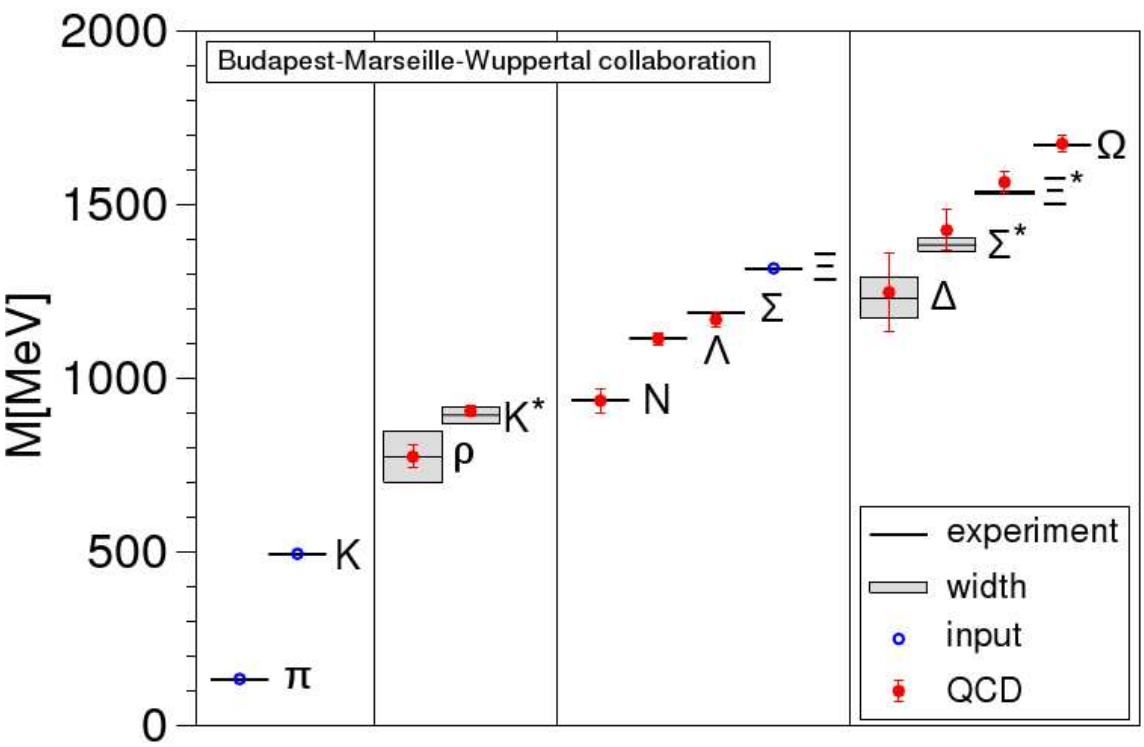
\includegraphics[width=.5\textwidth]{\PhDthesisdir/contents/chapter-MS-MSSM/formalisme/light_hadrons_masses.png}
\caption{Spectre de masse des hadrons légers. Les lignes horizontales ainsi que les zones grisées sont les valeurs expérimentales et les largeurs de désintégration. Les résultats issus de~\cite{ab_initio_hadron_masses} en utilisant des calculs de QCD sur réseau sont représentés par des cercles, avec les erreurs associées. Seules les masses des hadrons \pion, \Kaon\ et \Xibaryon\ sont sans barre d'erreur, elles sont utilisées pour fixer des paramètres libres du modèle.}
\label{fig-lattice_QCD_masses}
\end{figure}
\par La valeur de $g_s$ à une échelle d'énergie $k$ est reliée à la valeur de $g_s$ à une échelle d'énergie $\mu$ par la relation
\begin{equation}
g_s(k) = \frac{g_s(\mu)}{1+ \frac{11n_c-2n_f}{12\pi} g_s(\mu)\ln(\frac{k^2}{\mu^2})}
\end{equation}
avec $n_c$ le nombre de couleurs et $n_f$ le nombre de saveurs de quarks, \ie\ $n_c=3$ et $n_f=6$~\cite{salam2010elements}.
Cette relation peut ainsi se réécrire
\begin{equation}
g_s (k) =
\frac{6\pi}{21 \ln(\frac{k}{\Lambda_\text{QCD}})}
\msep
\Lambda_\text{QCD} = 218\pm\SI{24}{\MeV}
\mend[,]
\end{equation}
avec $\Lambda_\text{QCD}$ l'échelle d'énergie à laquelle $g_s$ diverge.
Il ressort que $g_s$ décroît lorsque l'échelle d'énergie augmente.
Cette diminution de $g_s$ aux hautes énergies est la \og liberté asymptotique \fg, régime où les particules colorées ne sont plus confinées et peuvent se propager comme des particules libres. Aux LHC, les énergies de collision permettent d'atteindre ce régime.
%the coupling decreases logarithmically, a phenomenon known as asymptotic freedom (the discovery of which was awarded with the Nobel Prize in Physics in 2004).
